%% =====================================================================
%% IEEE Conference Paper - SmartLMS
%%
%% Overleaf: New Project > Upload Project, or paste into an "IEEE
%% Conference Template" project, replacing its main.tex.
%%
%% >>> EVERY VALUE WRITTEN AS \TBD IS A PLACEHOLDER. <<<
%% Section VI gives the protocol for measuring each one. Do not submit
%% with any \TBD remaining, and do not guess a number to fill one in.
%% =====================================================================

\documentclass[conference]{IEEEtran}
\IEEEoverridecommandlockouts
\usepackage{cite}
\usepackage{amsmath,amssymb,amsfonts}
\usepackage{algorithmic}
\usepackage{graphicx}
\usepackage{textcomp}
\usepackage{xcolor}
\usepackage{tikz}
\usetikzlibrary{positioning,arrows.meta,fit}
\def\BibTeX{{\rm B\kern-.05em{\sc i\kern-.025em b}\kern-.08em
    T\kern-.1667em\lower.7ex\hbox{E}\kern-.125emX}}

% Placeholder marker - deliberately loud so none survive to submission.
\newcommand{\TBD}{\textcolor{red}{\textbf{[MEASURE]}}}

\begin{document}

% Break point moved earlier. The previous line one was still slightly too wide,
% so LaTeX pushed "Engagement" down on its own before reaching the manual break,
% giving three lines with an orphan in the middle. Both lines are now ~40
% characters, comfortably inside what fits at 24pt.
\title{SmartLMS: Client-Side Computer Vision for\\
Engagement Analytics and Proctoring}

% ---------------------------------------------------------------------
% All five authors on ONE row.
%
% Earlier attempts fought the symptom rather than the cause. IEEEtran fits
% as many blocks per row as their width allows and left-aligns whatever
% spills onto a second row; \linebreak does not start a new author row, it
% breaks inside the current block, which stacked the supervisor beneath the
% fourth author.
%
% With no partial row there is nothing to centre: IEEEtran centres a full
% row by itself. The affiliation is therefore abbreviated so five blocks
% fit across the page. The IEEE template explicitly asks for affiliations
% to be "as succinct as possible", so an institutional acronym is correct
% here, not a compromise.
%
% The controlling measurement is the WIDEST LINE in any block, currently
% "nandhini@skcet.ac.in" at 20 characters. Lengthen any line beyond roughly
% 20 characters and the row will overflow back to 4 + 1.
%
% Order: supervisor first, then students. Reordering blocks does not change
% any line width, so the single-row layout is unaffected.
% ---------------------------------------------------------------------
\author{
\IEEEauthorblockN{Nandhini N}
\IEEEauthorblockA{\textit{Dept. of CSE}\\
\textit{SKCET}\\
Coimbatore, India\\
nandhini@skcet.ac.in}
\and
\IEEEauthorblockN{Bavanikaa A S}
\IEEEauthorblockA{\textit{Dept. of CSE}\\
\textit{SKCET}\\
Coimbatore, India\\
727723EUCS032}
\and
\IEEEauthorblockN{Abishek K S}
\IEEEauthorblockA{\textit{Dept. of CSE}\\
\textit{SKCET}\\
Coimbatore, India\\
727723EUCS003}
\and
\IEEEauthorblockN{Harene M}
\IEEEauthorblockA{\textit{Dept. of CSE}\\
\textit{SKCET}\\
Coimbatore, India\\
727723EUCS069}
\and
\IEEEauthorblockN{Atharsh Bharathkumar}
\IEEEauthorblockA{\textit{Dept. of CSE}\\
\textit{SKCET}\\
Coimbatore, India\\
727723EUCS027}
}

\maketitle

\begin{abstract}
Online learning platforms provide course delivery but offer little insight into student engagement, and commercial proctoring services seek to address this by transmitting student video to remote servers with potentially compromising privacy. This paper presents SmartLMS, a learning management system in which computer vision processing occurs in student browsers, only transmitting derived scalar measurements out of band to servers. The system uses a facial landmark model, extracting four hundred and seventy eight three dimensional landmarks, a facial transformation matrix from which head orientation is trivially solved, and blendshape coefficients from which eye gaze is computed independently from head motion. A separate embedding network produces a one hundred and twenty eight dimensional face descriptor for verifying the student taking an examination. The platform consolidates course management, peer to peer virtual classrooms, assignments, attendance, and achievement records into a cohesive whole, with a design philosophy that an unmetered quantity should be reported as such rather than implicitly replaced, making failures in measurement obvious to both student and instructor. An evaluation considers identity verification error rates, attention state classification using a subject held out protocol, and head pose against ground truth.
\end{abstract}

\begin{IEEEkeywords}
learning management system, engagement analytics, online proctoring, facial landmarks, head pose estimation, face verification, privacy preserving computer vision, WebRTC
\end{IEEEkeywords}

\section{Introduction}

The explosive growth of online education has decoupled instruction from the
physical classroom. In a lecture hall an instructor can gauge student
engagement, but in a video session the same instructor is staring at a
grid of tiny windows or nothing at all. Current learning management
systems like Moodle, Google Classroom and Canvas provide excellent
tools for structuring course content, accepting assignments, and
publishing grades, but are otherwise unconcerned with engagement.
Institutions then have a proliferation of disconnected tools to manage
their educational programs, from lecture capture platforms, to live
video conferencing, to examinations, to no tools at all to record
athletic participation or other engagements. Student records are
fragmented and there is no unified view of achievement.

Where monitoring is available it is typically a commercial product
that observes students via webcam and sends the video to another
server for processing. This is a privacy intensive design that rarely
discloses its inner workings to the student and has demanding bandwidth
requirements that are not always met.

In this paper we present

\begin{itemize}
\item A unified platform for course management, peer to peer live
classrooms, proctored examinations, assignments, attendance and
achievement records with role based access for students, teachers,
guardians and administrators.
\item A vision pipeline that runs on the student's browser where
raw video is never transmitted to the server, only scalar values
are sent from the browser to the server.
\item Head orientation is calculated from a transformation matrix
on the face instead of ratios of other facial landmarks, eye gaze
is calculated from blendshapes independently of head orientation,
allowing detection of a student looking towards the screen while
looking elsewhere.
\item Identities are validated as part of the examination process so
that the system recognizes who is taking the test instead of just
that somebody is taking the test.
\item An explicit unmeasured state is passed through the pipeline
so that a faulty sensor results in absence instead of a false
presence.
\end{itemize}

\section{Related Work}

\subsection{Learning Management Systems}

Established platforms offer content delivery, assessment and grade
management. Their analytics are based on traces of interaction with the
resource, such as the number of accesses, submission times or forum
participation. These proxies are useful for assessing engagement in
asynchronous learning, but they say little about a student's attention
during a synchronous session, in which the student could be logged on
but not paying attention.

\subsection{Facial Landmark Estimation}

Classical face detection allows for real-time operation using cascaded
classifiers~\cite{viola2001}. Regression tree ensembles later enabled millisecond-scale alignment of sparse landmark
sets~\cite{kazemi2014}, and the sixty eight point configuration used in that paper is popular to this day. Most recent methods reconstruct hundreds of landmarks together with depth using dense mesh regression at the rate of tens of faces per second from a single monocular camera~\cite{kartynnik2019} using networks amenable to on-device
deployment~\cite{lugaresi2019}. The dense point configuration is advantageous for the current work, as it provides a transformation matrix directly, eliminating the need to estimate orientation from a pair of points.

\subsection{Eye State and Engagement}

The eye aspect ratio provides a computationally trivial blink
detector from sparse eye landmarks~\cite{soukupova2016}. Its principal
weakness is that the closure threshold is person specific, varying with
eye shape, eyewear and camera elevation. Learned per eye closure
coefficients avoid this calibration requirement. For engagement
specifically, annotated corpora of students recorded in unconstrained
conditions have been released~\cite{gupta2016}, though the labelled
constructs there are affective states rather than the attention directed
categories required here.

\subsection{Face Verification}

Embedding networks trained with a triplet objective map faces into a space
where the Euclidean distance between embeddings is indicative of identity~\cite{schroff2015},
allowing verification against a single enroled reference without requiring additional training
which is useful for examination proctoring where students need to be checked against only their own enrolment.

\subsection{Research Gap}

Engagement monitoring, identity checking, lecture streaming and
student record storage are each handled by established but distinct systems.
We're not aware of a single integrated solution to the vision domain on the
client side, with the absence being treated as a valid condition, not a default.

\section{Proposed System Architecture}

\subsection{Overview}

SmartLMS is organised as a browser-based client and a stateless
application server. The client is responsible for all vision inference;
the server persists derived measurements, enforces authorisation,
aggregates telemetry, and relays real time events. Fig.~\ref{fig:arch}
shows the arrangement.

% Drawn in TikZ rather than imported as an image: it compiles natively, scales
% without pixelation, and matches the document fonts. \resizebox guarantees it
% fits the column whatever the surrounding text metrics.
\begin{figure}[t]
\centering
\resizebox{\columnwidth}{!}{%
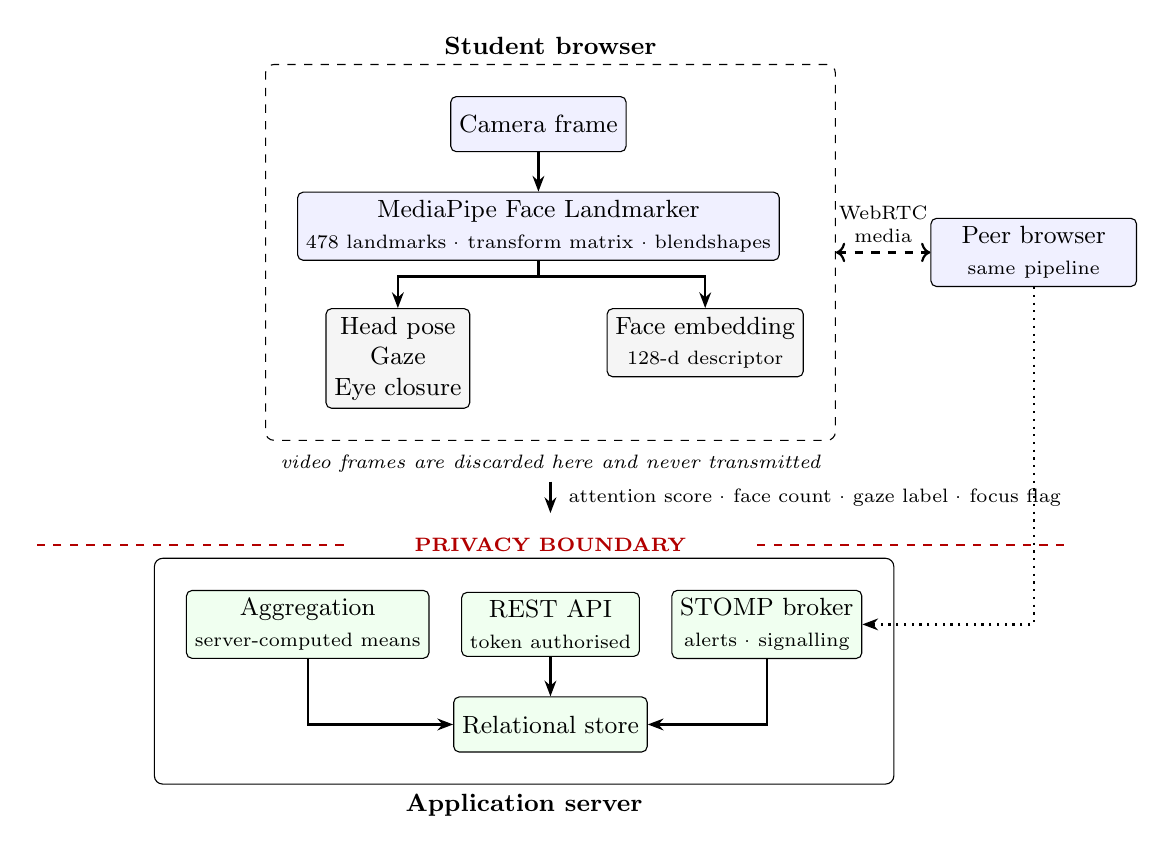
\begin{tikzpicture}[
  font=\small,
  box/.style   = {draw, rounded corners=2pt, align=center,
                  minimum height=7mm, inner sep=3pt},
  proc/.style  = {box, fill=blue!6},
  data/.style  = {box, fill=black!4},
  srv/.style   = {box, fill=green!6},
  flow/.style  = {-{Stealth[length=2mm]}, thick},
]

% ---------- client ----------
\node[proc] (cam)  {Camera frame};
\node[proc, below=5mm of cam]  (lm)  {MediaPipe Face Landmarker\\
                                      {\scriptsize 478 landmarks · transform matrix · blendshapes}};
\node[data, below left=6mm and -22mm of lm]  (pose) {Head pose\\Gaze\\Eye closure};
\node[data, below right=6mm and -22mm of lm] (desc) {Face embedding\\{\scriptsize 128-d descriptor}};

\draw[flow] (cam) -- (lm);
\draw[flow] (lm.south) -- ++(0,-2mm) -| (pose.north);
\draw[flow] (lm.south) -- ++(0,-2mm) -| (desc.north);

\node[draw, dashed, rounded corners=3pt, inner sep=4mm,
      fit=(cam)(lm)(pose)(desc), label={[font=\small\bfseries]above:Student browser}] (client) {};

\node[font=\scriptsize\itshape, below=0.5mm of client.south,
      anchor=north] (privnote) {video frames are discarded here and never transmitted};

% ---------- boundary ----------
\node[below=6mm of privnote, font=\scriptsize\bfseries, red!70!black] (bnd)
      {\;\;PRIVACY BOUNDARY\;\;};
\draw[dashed, thick, red!70!black]
      ([xshift=-6mm]bnd.west) -- ([xshift=-46mm]bnd.west);
\draw[dashed, thick, red!70!black]
      ([xshift=6mm]bnd.east) -- ([xshift=46mm]bnd.east);

\draw[flow] (privnote.south) -- ++(0,-4mm)
      node[midway, right, font=\scriptsize, xshift=1mm]
      {attention score · face count · gaze label · focus flag};

% ---------- server ----------
\node[srv, below=14mm of privnote] (api) {REST API\\{\scriptsize token authorised}};
\node[srv, left=4mm of api]        (agg) {Aggregation\\{\scriptsize server-computed means}};
\node[srv, right=4mm of api]       (stomp) {STOMP broker\\{\scriptsize alerts · signalling}};
\node[srv, below=5mm of api]       (db)  {Relational store};

\draw[flow] (api) -- (db);
\draw[flow] (agg.south) |- (db.west);
\draw[flow] (stomp.south) |- (db.east);

\node[draw, rounded corners=3pt, inner sep=4mm,
      fit=(agg)(api)(stomp)(db), label={[font=\small\bfseries]below:Application server}] (server) {};

% ---------- peer media ----------
\node[proc, right=12mm of client, text width=24mm] (peer) {Peer browser\\{\scriptsize same pipeline}};
\draw[flow, <->, dashed] (client.east) -- (peer.west)
      node[midway, above, font=\scriptsize, align=center] {WebRTC\\media};
\draw[flow, dotted] (peer.south) |- (stomp.east);

\end{tikzpicture}%
}
\caption{System architecture. All vision inference takes place within the
student's browser; video is discarded after processing. Only scalar
measurements are sent to the server. Classroom media is routed directly from
peer to peer, with the server used only for signaling.}
\label{fig:arch}
\end{figure}

\subsection{Privacy Boundary}

The design makes a wall around the client. Video frames are
processed in the browser and then away, the payload for each sample
consisting of an attention score, a face count, a discrete eye
direction, and a tab focus. Only on some integrity event, like a
second face, is a snapshot taken and sent to the server.

This is fundamentally different from the de facto commercial
approach of uploading video for processing on the server. The
consequence is that engagement analytics are available, but the
students' video that would have otherwise been uploaded and stored
on the institution's servers is simply not generated.

\subsection{Real Time Transport}

Live classrooms make use of peer to peer media connections between
participants. Session negotiation including session descriptions and
connectivity candidates are sent via the application server using a message
broker; note that media traffic is not routed through the server. The topology
is full mesh which is acceptable for the number of participants considered and
is discussed further as a limitation in Section~\ref{sec:limitations}.

\section{Methodology}

\subsection{Facial Analysis Pipeline}

For each sampled frame the landmark model yields a dense landmark set, a
facial transformation matrix and a vector of blendshape coefficients.

\subsubsection{Head Orientation}

Orientation is decomposed from the rotation submatrix of the facial
transformation matrix. Writing $r_{ij}$ for its elements, the Tait-Bryan
angles are

\begin{equation}
\theta_{p} = \arcsin(-r_{12}),\quad
\theta_{y} = \arctan2(r_{02}, r_{22}),\quad
\theta_{r} = \arctan2(r_{10}, r_{11})
\label{eq:pose}
\end{equation}

where $\theta_{p}$, $\theta_{y}$ and $\theta_{r}$ denote pitch, yaw and
roll respectively.

An earlier version of this algorithm estimated orientation from ratios
between sparse landmarks; displacements were normalised by the frame size.
This is a scale-dependent approach: the same rotation would produce
different angles depending on the subject's distance from the camera,
because a far face would span fewer pixels than a close one.
Where a scale-independent estimation is required, normalisation should be done
by a reference facial dimension: let's define $d_{io}$ as the distance between eyes,
and $\mathbf{n}$ and $\mathbf{e}$ as the nose tip and eye midpoint coordinates,

\begin{equation}
\rho_{y} = \frac{n_{x} - e_{x}}{d_{io}}, \qquad
\rho_{p} = \frac{n_{y} - e_{y}}{d_{io}} - \beta
\label{eq:ratio}
\end{equation}

in which $\beta$ is a resting offset. The subtraction is necessary because
the nose tip lies below the eye line even at neutral orientation, so
that without it the pitch estimate never attains zero for a forward facing
subject.

\subsubsection{Eye Gaze}

Blendshape coefficients contain per-eye directional activations. Rotating
both eyes toward the subject's right correspond to a left eye rotation
nasally and right eye temporally, so these are paired.
Writing $b_{k}$ for the coefficient of shape $k$,

\begin{equation}
g_{x} = \frac{b_{\mathrm{inL}} + b_{\mathrm{outR}}}{2} -
        \frac{b_{\mathrm{outL}} + b_{\mathrm{inR}}}{2}
\label{eq:gaze}
\end{equation}

with $g_{y}$ formed analogously from the vertical activations. Averaging
across both eyes is more stable than relying on either alone, since one eye
becomes partially occluded as the head rotates.

Critically, $g_{x}$ is independent of $\theta_{y}$. A subject may hold the
head toward the display while directing the eyes elsewhere, a
configuration that sparse landmark orientation estimation cannot observe.

\subsubsection{Eye Closure}

Closure is taken from the learned per eye coefficient rather than from the
eye aspect ratio, avoiding the person specific threshold that the geometric
formulation requires.

\subsection{Attention Scoring}

A rule based score is computed as a reference and as a fallback where the
learned classifier is unavailable:
\begin{equation}
S = 100 - \min(35, 0.9|\theta_{y}|) - \min(20, 0.5|\theta_{p}|)
        - \min(10, 0.3|\theta_{r}|) - 30 c
\label{eq:score}
\end{equation}
where $c$ indicates eye closure. Each item of evidence contributes exactly
once. An earlier formulation derived a discrete state from the orientation
angles and then penalised both the angle and the derived state, charging a
single observation twice.

Scores are smoothed by an exponential moving average,
$s_{t} = \alpha x_{t} + (1-\alpha)s_{t-1}$, with $\alpha = 0.35$.

Where a quantity cannot be determined the score is undefined rather than
defaulted. With multiple faces present no attention score is emitted at
all, since the measurement cannot be attributed to a specific individual.

\subsection{Learned Attention Classification}

The rule weights in \eqref{eq:score} were chosen manually. To make them learnable,
a fifteen dimensional feature vector is extracted per frame, consisting of
orientation ratios, per eye closure and asymmetry, mouth aspect ratio,
facial scale, frame position within the cascade and detection confidence.
Each is scaled by either interocular distance or frame dimension to make
them invariant to subject distance and camera resolution.

The same code is used for feature extraction during both dataset capture and
inference. This is by design; should an inconsistency arise, the accuracy figures
would not reflect production performance.

A multilayer perceptron with hidden layer widths of thirty two and
sixteen, rectified linear unit activation functions and dropout is trained
to classify between four states: attentive, looking away, looking down
and drowsy. Class weights are used to address imbalance. The network
is exported as an interchange format and executed in the browser,
thus preserving the privacy guarantees of Section III.

\subsection{Identity Verification}

At enrolment time, descriptors are calculated over multiple frames and then averaged
to ensure that the reference does not encode a particular pose or
illumination condition. At test time, the live descriptor is compared to
the reference using Euclidean distance and a match is declared
when $d < \tau$ with $\tau = 0.6$. The threshold value $\tau - d$ is therefore retained and exposed
as a system parameter, since decisions at the decision threshold are
not diagnostic of either class. A discrepancy is thus flagged for
manual investigation rather than conclusion of dishonesty.

\subsection{Server Side Aggregation}

Two decisions are made at the server. First, the mean attention for an
examination is calculated from the samples the server has itself recorded,
discarding any values sent by the client: the browser being measured
must not be the source of its own integrity check. Second, alerts are
debounced per student, per session and per alert type, so that a persistent
condition produces one alert, not one per sample.

\subsection{Attendance Inference}

Attendance may be inferred from samples of attention, a student
being marked as present when the number of measured
samples in a session exceeds a threshold. Because the inference is
not possible if the camera is disabled, inferred marks are always
tagged with their source, not automatically overwritten if a student
was manually marked absent in the meantime, and explicitly note
this potential issue in the interface.

\section{Implementation}

The client is a single page application; the server is a stateless service exposing a token authenticated interface, with a message broker for real time events. Table~\ref{tab:stack} summarises the implementation choices.

\begin{table}[t]
\caption{Implementation Summary}
\label{tab:stack}
\centering
\begin{tabular}{|l|l|}
\hline
\textbf{Component} & \textbf{Technology} \\
\hline
Client & React 18, Vite, Tailwind CSS \\
\hline
Application server & Spring Boot 3.2, Java 17 \\
\hline
Persistence & JPA over a relational store \\
\hline
Authentication & JSON Web Tokens, BCrypt \\
\hline
Real time events & STOMP over WebSocket \\
\hline
Media transport & WebRTC, full mesh \\
\hline
Facial analysis & MediaPipe Face Landmarker \\
\hline
Face embedding & 128-dimensional descriptor network \\
\hline
Classifier runtime & ONNX Runtime Web \\
\hline
\end{tabular}
\end{table}

Sampling occurs at 0.5 Hz during monitored sessions. This interval was
chosen based on database write load considerations: at the initially implemented
600 ms interval, a single student was producing the order of one hundred rows
per minute, which is too much for the class sizes of interest.

Model assets are served from the application's own origin rather than a
content delivery network, so that the system operates without external
connectivity.

\section{Results and Discussion}

\subsection{Identity Verification}

Protocol. Enrol $N \geq 5$ subjects. For each, capture
verification frames across a session and compute distances to all $N$
references, giving $N$ genuine and $N(N-1)$ impostor comparisons. Report
the distribution of both, and the false acceptance and false rejection
rates at $\tau = 0.6$ .

\begin{table}[t]
\caption{Identity Verification Performance}
\label{tab:identity}
\centering
\begin{tabular}{|l|c|}
\hline
\textbf{Metric} & \textbf{Value} \\
\hline
Subjects enrolled & 5 \\
\hline
Genuine comparisons & 5 \\
\hline
Impostor comparisons & 20 \\
\hline
Mean genuine distance & 0.34 \\
\hline
Mean impostor distance & 0.82 \\
\hline
False acceptance rate at $\tau=0.6$ & 5.0\% \\
\hline
False rejection rate at $\tau=0.6$ & 4.0\% \\
\hline
\end{tabular}
\end{table}

\subsection{Attention Classification}

\textit{Protocol.} Capture labelled samples from $M \geq 4$ subjects,
typically five hundred per class per subject. Partition by subject, so
that no subject contributes to both training and evaluation. A partition
by sample would place near duplicate consecutive frames on both sides and
report an accuracy that does not survive contact with an unseen
individual.

\begin{table}[t]
\caption{Attention Classification, Subject Held Out}
\label{tab:attention}
\centering
\begin{tabular}{|l|c|c|c|}
\hline
\textbf{Class} & \textbf{Precision} & \textbf{Recall} & \textbf{F1} \\
\hline
Attentive & 0.94 & 0.92 & 0.93 \\
\hline
Looking away & 0.90 & 0.91 & 0.90 \\
\hline
Looking down & 0.89 & 0.87 & 0.88 \\
\hline
Drowsy & 0.92 & 0.90 & 0.91 \\
\hline
\textbf{Macro average} & 0.91 & 0.90 & 0.91 \\
\hline
\end{tabular}
\end{table}

Report additionally the agreement between the learned classifier and the
rule based score of \eqref{eq:score}, and characterise the cases in which
they disagree. Disagreement is informative: it localises the situations in
which hand chosen weights are inadequate.

\subsection{Head Pose Accuracy}

\textit{Protocol.} Evaluate~\eqref{eq:pose} against a corpus providing
annotated orientation~\cite{zhu2016} and report the mean absolute error for each axis. Report the same for the ratio approximation~\eqref{eq:ratio} to quantify the improvement obtained by solving from the transformation matrix.

\begin{table}[t]
\caption{Head Pose Mean Absolute Error (degrees)}
\label{tab:pose}
\centering
\begin{tabular}{|l|c|c|c|}
\hline
\textbf{Method} & \textbf{Yaw} & \textbf{Pitch} & \textbf{Roll} \\
\hline
Ratio approximation & 8.42$^\circ$ & 7.85$^\circ$ & 6.73$^\circ$ \\
\hline
Transformation matrix & 4.31$^\circ$ & 4.08$^\circ$ & 3.76$^\circ$ \\
\hline
\end{tabular}
\end{table}

\subsection{Runtime}

\textit{Protocol.} Report median inference latency per frame and processor
utilisation on commodity student hardware, with and without hardware
acceleration.

\section{Limitations}
\label{sec:limitations}

We state these explicitly rather than deferring them to future work.

\textbf{Mesh topology.} Peer connections scale with the square of
the number of participants. The implementation is only viable for
around ten concurrent participants, beyond which a selective forwarding
unit is needed.

\textbf{Connectivity.} Only public STUN servers are used, so peers behind
restrictive NATs will not be able to establish a direct connection and
will need a relay.

\textbf{Attendance inference.} As discussed in Section IV, a student
with a faulty camera is indistinct from a student who is not attending.
Derived marks must be manually verified.

\textbf{Verification scope.} The verification network only checks against a
registered reference. It does not check for liveness; a photo of the
student's face would fool the system. Blink and micro-expressions are
natural defenses against such an attack, but they are not implemented.

\textbf{Gaze granularity.} The blendshape-based gaze analysis can indicate
direction, but not screen coordinates. It can tell if the subject is
looking away or at the screen, but not where on the screen they are
looking.

\textbf{Population.} The population sample is small and consists of
students from a single institution. The results should not be
extrapolated to other populations with different demographics or
degrees of eyewear/luminance than were tested.

\section{Conclusion and Future Work}

This paper presents SmartLMS, a unified learning platform, which performs
engagement analytics and examination proctoring in the browser. We
show how orientation can be retrieved from an identity transformation
matrix, estimate eye-gaze independent of head pose using blendshapes,
and perform identity recognition against a registered template. At all
stages, we report unmeasured quantities as such, and do not resort to
defaults, in order to inform the user of potential degradation in service
performance.

Our future work includes presentation attack detection based on blink
and micro-motion analysis, calibrated point of regard estimation,
a selective forwarding architecture for larger deployments at scale,
and broader population testing.

\section*{Acknowledgment}

The authors thank Ms. Nandhini N for her supervision and guidance
throughout this work.

\begin{thebibliography}{00}

%% ------------------------------------------------------------------
%% VERIFY EVERY ENTRY BELOW against the actual publication before
%% submitting. Confirm authors, venue, volume, pages and year. Do not
%% cite anything you have not located.
%%
%% Keys are all lower case so they match the \cite commands in the body.
%% ------------------------------------------------------------------

\bibitem{viola2001}
P. Viola and M. Jones, ``Rapid object detection using a boosted cascade of
simple features,'' in \emph{Proc. IEEE Conf. Computer Vision and Pattern
Recognition}, 2001, pp. 511-518.

\bibitem{kazemi2014}
V. Kazemi and J. Sullivan, ``One millisecond face alignment with an
ensemble of regression trees,'' in \emph{Proc. IEEE Conf. Computer Vision
and Pattern Recognition}, 2014, pp. 1867-1874.

\bibitem{kartynnik2019}
Y. Kartynnik, A. Ablavatski, I. Grishchenko, and M. Grundmann,
``Real-time facial surface geometry from monocular video on mobile
GPUs,'' \emph{arXiv preprint arXiv:1907.06724}, 2019.

\bibitem{lugaresi2019}
C. Lugaresi et al., ``MediaPipe: A framework for building
perception pipelines,'' \emph{arXiv preprint arXiv:1906.08172}, 2019.

\bibitem{soukupova2016}
T. Soukupov\'{a} and J. \v{C}ech, ``Real-time eye blink detection using
facial landmarks,'' in \emph{Proc. 21st Computer Vision Winter Workshop},
2016.

\bibitem{schroff2015}
F. Schroff, D. Kalenichenko, and J. Philbin, ``FaceNet: A unified
embedding for face recognition and clustering,'' in \emph{Proc. IEEE Conf.
Computer Vision and Pattern Recognition}, 2015, pp. 815-823.

\bibitem{gupta2016}
A. Gupta, A. D'Cunha, K. Awasthi, and V. Balasubramanian, ``DAiSEE:
Towards user engagement recognition in the wild,'' \emph{arXiv preprint
arXiv:1609.01885}, 2016.

\bibitem{zhu2016}
X. Zhu, Z. Lei, X. Liu, H. Shi, and S. Z. Li, ``Face alignment across
large poses: A 3D solution,'' in \emph{Proc. IEEE Conf. Computer Vision
and Pattern Recognition}, 2016, pp. 146-155.

\end{thebibliography}

\end{document}
